\documentclass[12pt]{article}
\usepackage[paperwidth=188.88mm,paperheight=246mm,textwidth=427.64493pt,textheight=596.5pt,centering]{geometry}
\usepackage{graphicx}
\usepackage{subcaption}
\usepackage[T1]{fontenc}
\captionsetup{font=small,skip=2pt}
\pagestyle{empty}
\setlength{\parindent}{0pt}
\begin{document}
{\small\textbf{Publication style specimen}\hfill Saved results only}\par
\vspace{3pt}
\begin{minipage}{\linewidth}\captionsetup{type=figure}
\begin{subfigure}[t]{.49\linewidth}
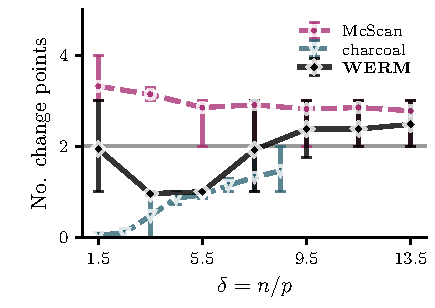
\includegraphics[width=\linewidth]{m2_counts.pdf}
\caption*{(a) M2: selected counts.}
\end{subfigure}\hfill
\begin{subfigure}[t]{.49\linewidth}
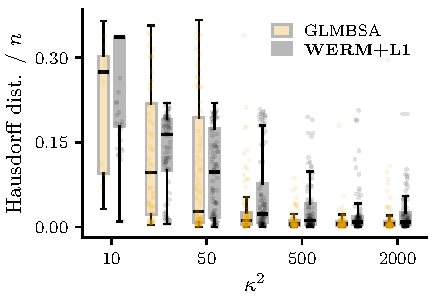
\includegraphics[width=\linewidth]{m3_location.pdf}
\caption*{(b) M3: localization.}
\end{subfigure}
\end{minipage}\par\vspace{4pt}
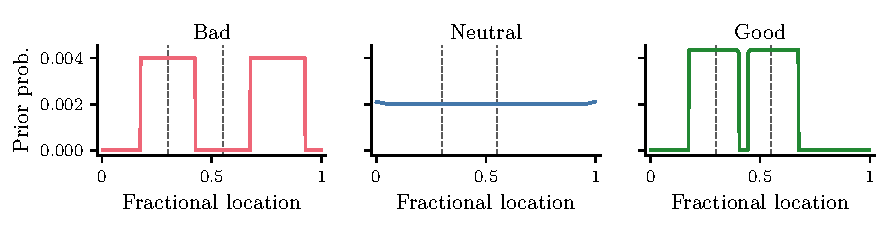
\includegraphics[width=\linewidth]{prior_triptych.pdf}
\par{\small (c) E-PRIOR: exact pooled change-point location prior.}\par
\vspace{3pt}
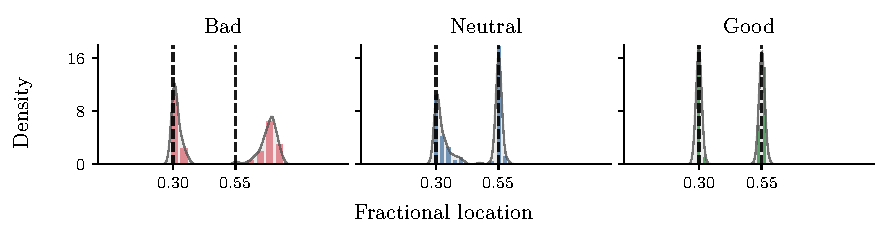
\includegraphics[width=\linewidth]{location_histograms.pdf}
\par{\small (d) E-PRIOR: estimated locations; dashed lines mark truth.}\par
\vspace{3pt}
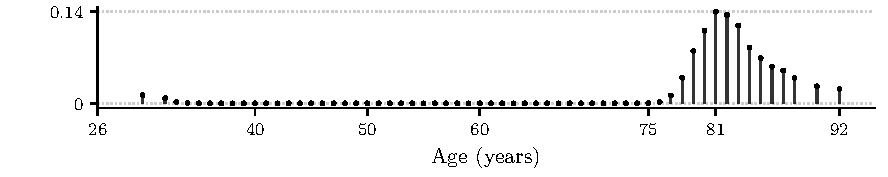
\includegraphics[width=\linewidth]{myocardial_posterior.pdf}
\par{\small (e) Myocardial: posterior conditional on one change point.}\par
\vspace{5pt}
{\footnotesize Fixed canvases at manuscript text width; Computer Modern;
axis labels 10.5\,pt, ticks 8.5\,pt. View at actual size to assess typography.
}
\end{document}
